\chapter{Point Cloud Analysis} \label{ch:analysis_pc}
In this chapter the point clouds are looked at in more detail on a local per-point scale, including the dispersion pattern of points on the surfaces. Some local measures will be defined that assign to each point in the point cloud a value in relation with its surrounding points. A way to predict the dispersion of points will be developed.

\section{Local density}
The \emph{local surface density} $\rho(p)$ of a point cloud $P$ around a point $p \in P$ indicates how densely points are dispersed on the surface around $p$, expressed in number of points per surface area. Because the shape of the underlying surface is unknown, a precise measure cannot be defined, and instead an approximation is used.

Taking the $k$ nearest neighbors around a point $p$ that is in a region where the surface is approximately planar results in a set of points located approximately on a disk around $p$. In this case, an estimate for the density is $\rho(p) = \frac{k}{\pi \, r_{\text{max}}^2}$, where $r_{\text{max}}$ is the maximal distance of one of the neighbors to $p$.

Even when the surface is not locally planar in that region, some level of accuracy is retained because Euclidian distances in three-dimensional space are measured, which are approximatively (on the scale of inter-point distances) equal to distances measured along the surface on which the disk would be wrapped.

Using $r_{\text{max}}$ makes the measure more sensitive to outliers, and can overestimate the density: $r_{\text{max}}$ by definition is the smallest least radius such that $k$ points are inside the disk. An alternative is to use the median $r_{\text{med}}$ of the radii, and set $\rho(p) = \frac{k}{2 \, \pi \, r_{\text{med}}^2}$. For the median value, half of the $k$ points have a smaller radius and are thus inside the disk.

When the density is supposed to be constant for each point in the point cloud, it will also be denoted as $\rho$ or $\rho(P)$.

\subsection{Square grid density}
For artificially generated point clouds, per-point densities $\rho(p)$ are set to their theoretical values. For a planar surface where points are arranged on a square grid with side length $l$, this density is $\rho(p) = \frac{1}{l^2}$, because $1$ point can be counted per square. This will be extended to parallelogram grids in the next chapter.


\section{Local curvature} \label{sec:curvature}
In the rest of this chapter, properties of the dispersion of points on planar surfaces of the model will be used. It is therefore important to distinguish between approximatively planar regions of the surface, and more sharp edges.

Unlike the density, this is a measure of the surface and not of the point dispersion on it. This implies that the metric should be invariant of the point dispersion. In addition to this, it is dependent on a scale parameter: for example a point cloud representing a wall of a building would be planar on a scale of a few centimeters, but not on a millimeter scale where the texture of the wall is considered.

A measure of \emph{local curvature} $c(p, r)$ around a point $p \in P$ with a radius $r \in \mathbb{R}$ will be defined. A tangent plane is attached to the point $p$, with the same normal vector $\vec{n}$ as the point. This normal vector is assumed to have been calculated beforehand. Then it is measured how well the neighboring points fit on the plane.

Using the local density $\rho(p)$, the expected number of points located in a radius $r$ on the surface is $\rho(p) \, \pi \, r^2$. Using a kNN algorithm the $k = \lceil \rho(p) \, \pi \, r^2 \rceil$ nearest neighbors $N_k \subset P$ are searched. When $k$ is below a predefined threshold it is increased to a minimal value. This is for example the case on oblique surfaces where the density is lower and the nearest neighbor distances get larger.

If the surface is locally planar around and $p$ in the given radius, the points $N_k$ will be located in a disk around $p$, with a radius of approximatively $r$. Because the circumference of a circle is proportional to its radius, $N_k$ contains more points at higher radii, and the probability density of their distance to $p$ increases linearly. But these points at a higher distance that fit on the plane should not overcompensate for nearer points that don't. Weights are attributed to the points to cancel out that effect: The weight of the closest point $p_1$ is set to $1$, and those of the remaining points $p_i$ to $\frac{\| p_1 - p \|}{\| p_i - p \|}$. Then the weights are normalized to sum up to $1$.

To measure how well a point $p_i \in N_k$ fits the plane, two values are useful: Its unsigned distance $|d_i|$ to the plane, and the absolute angle $|\alpha_i|$ between its normal vector $\vec{n_i}$ and that of the plane $\vec{n}$. Both can be calculated using the dot products:
\begin{equation}
d_i = \vec{n} \, (\vec{p_i} - \vec{p})
\hspace{7mm} \text{and} \hspace{7mm}
\cos \alpha_i = \vec{n} \, \vec{n_i}
\end{equation} 

The local curvature metric is calculated as weighted average of those values for the $k$ neighboring points:
\begin{equation}
c(p, r) = \frac{1}{k} \sum_{i=1}^{k} w_i \, \left( A \, |\alpha_i| + D \, |d_i| \right)
\end{equation}
where the coefficients $A$ and $D$ are set so as to attribute different weights to the two measures. To avoid evaluating $\arccos$ for each point, the angle can be approximated using $\alpha'_i = \frac{\pi}{2} (1 - \vec{n} \, \vec{n_i})$. These two figures show two surfaces (in two dimensions) where one metric it high and the other low.
\begin{figure}[H]
\centering
\begin{subfigure}{.4\textwidth}
	\includegraphics[width=\linewidth]{fig/curvature_distances.pdf}
	\caption{Large $\sum |d_i|$, small $\sum |\alpha_i|$}
\end{subfigure}%
\hspace{15mm}%
\begin{subfigure}{.4\textwidth}
	\includegraphics[width=\linewidth]{fig/curvature_angles.pdf}
	\caption{Large $\sum |\alpha_i|$, small $\sum |d_i|$}
\end{subfigure}	
\end{figure}
For the purposes that the curvature measure is used here, $A$ should be set higher, because surfaces such as the left-side one can still be considered locally planar.

In figure \ref{fig:curvature_example} the ``dessus-de-porte'' scan is shown with points colorized according to this curvature measure. The color scale is shown on the figure. The blue and green parts indicate lower curvature, and thus more planar surface. It can be seen that the straight wall in the background is identified as being more planar, while rounded surfaces on the stone figures get a higher curvature value. Here $A = 10$ and $D = 3$, and $r = 0.01$ is used. The scale ranges from $c(p, r) = 0.000$ to $0.003$.


\begin{figure}[h]
\centering
\includegraphics[width=.7\textwidth]{fig/curvature_example.png}
\caption{Example point cloud colorized according to curvature measure}
\label{fig:curvature_example}
\end{figure}

\FloatBarrier

\section{Point dispersion}
Point dispersion here refers to how points in a point clouds are arranged on a surface. When the surface is locally planar, regions of the surface can be approximated by a plane. The following three point dispersions on the plane will be analyzed:
\begin{figure}[H]
\centering
\hspace*{\fill}%
\begin{subfigure}{.3\textwidth}
{
	\setlength{\fboxsep}{0pt}%
	\setlength{\fboxrule}{0.5pt}%
	\fbox{\includegraphics[width=\linewidth]{fig/dispersion_random.png}}%
	\caption{Random dispersion}
}
\end{subfigure}%
\hfill%
\begin{subfigure}{.3\textwidth}
{
	\setlength{\fboxsep}{0pt}%
	\setlength{\fboxrule}{0.5pt}%
	\fbox{\includegraphics[width=\linewidth]{fig/dispersion_sqgrid.png}}%
	\caption{Square grid}
}
\end{subfigure}%
\hfill%
\begin{subfigure}{.3\textwidth}
{
	\setlength{\fboxsep}{0pt}%
	\setlength{\fboxrule}{0.5pt}%
	\fbox{\includegraphics[width=\linewidth]{fig/dispersion_pargrid.png}}%
	\caption{Parallelogram grid}
}%
\end{subfigure}\\
\caption{Different point dispersions on planar surface}
\label{fig:point_dispersion}
\end{figure}

The \emph{random dispersion} is the most general case, where the $x$ and $y$ coordinates of each points are independent, random variables, with a uniform distribution. It can be seen visually that the local density in that case is not constant.

Point clouds recorded by a laser scanner will produce a dispersion that is more akin to the \emph{square grid dispersion}. If the scanner processes in sequential scan-lines, and uses a regular graduation of azimuth and elevation coordinates, a planar surface placed perpendicular to the scanner ray will \emph{locally} get points approximatively arranged in squares. The dispersion will be considered to be invariant to a two-dimensional rotation of the plane itself.

Here the terms ``grid'' and ``lattice'' to describe the patterns that the points form on the surface, will be used interchangeably. Lattice is the mathematical proper term, grid emphasizes that the points get connected on two axis.

\subsection{Parallelogram grid}
When the surface is placed at an oblique angle to the scanner line, the points on the plane will instead be dispersed on a \emph{parallelogram grid}. Figures \ref{fig:closeup_ddp}, \ref{fig:closeup_wall} show two close-up views from the ``Hôtel de Ville'' scans, featuring the parallelogram grid point dispersion on approximatively planar surfaces. Figure \ref{fig:bunny_grid_closeup} is taken from the Stanford Bunny point cloud, which was also recorded using a laser scanner. A square grid or rectangular grid are special case of this.

\begin{figure}[h]
\centering
\includegraphics[width=.5\textwidth]{fig/closeup_ddp.png}
\caption{Closeup of the surface distribution of points on front wall of building}
\label{fig:closeup_ddp}
\end{figure}

\begin{figure}[h]
\centering
\includegraphics[width=.5\textwidth]{fig/closeup_wall.png}
\caption{Closeup of the surface distribution of points on detail of front wall}
\label{fig:closeup_wall}
\end{figure}

\begin{figure}[h]
\centering
{
	\setlength{\fboxsep}{0pt}%
	\setlength{\fboxrule}{0.5pt}%
	\fbox{\includegraphics[width=.4\textwidth]{fig/bunny_grid_closeup.png}}
}
\caption{Closeup of the surface distribution of points on Bunny point cloud}
\label{fig:bunny_grid_closeup}
\end{figure}


The diagram on figure \ref{fig:pargrid_proj} shows the parallel projection of a square from camera image space onto a plane in three-dimensional space. $\vec{n}$ is the normal vector of the plane, $p_l$ the width and height (side length) of the square, and $x, y$ the corresponding side lengths of the projected square. It can be seen that the projected square takes on the shape of a parallelogram on the plane. This models the projection of scanner rays on a surface. The coordinate system is such that the scanner is placed at origin. Since only a small region of a locally planar surface is considered (compared to the field of view of the scanner), adjacent rays in azimuth and elevation direction are modeled as parallel. When the square is extended to form a square grid in the XY-plane, a parallelogram grid is formed on the plane in which all parallelograms have the same two side lengths and inner angles.

\begin{figure}[h]
\centering
\includegraphics[width=.3\textwidth]{fig/pargrid_proj.png}
\caption{Parallel projection of square onto plane in space}
\label{fig:pargrid_proj}
\end{figure}

As can be seen on figure \ref{fig:par_grid_tilings}, several different parallelogram grids are possible for the same dispersion of points on the plane. The two grids in these examples have no sides in common. The projection of the camera square grid on the plane results in one of the possible parallel grids. When the plane is placed at a more oblique angle from the camera, it tends to be a grid with longer side lengths, like as the second one on the figure. It is generally not such that it includes the shortest possible parallelogram edge.

The ``parallelogram grid'' is described mathematically as a lattice in $\mathbb{R}^2$. The projections of $\vec{x} = \transpose{(p_l, 0)}$ and $\vec{y} = \transpose{(0, p_l)}$ from the camera image constitute one of the infinitely many possible bases for this lattice. \cite{Galb2012}

\begin{figure}[h]
\centering
\hspace*{\fill}%
\begin{subfigure}{.3\textwidth}
{
	\setlength{\fboxsep}{0pt}%
	\setlength{\fboxrule}{0.5pt}%
	\fbox{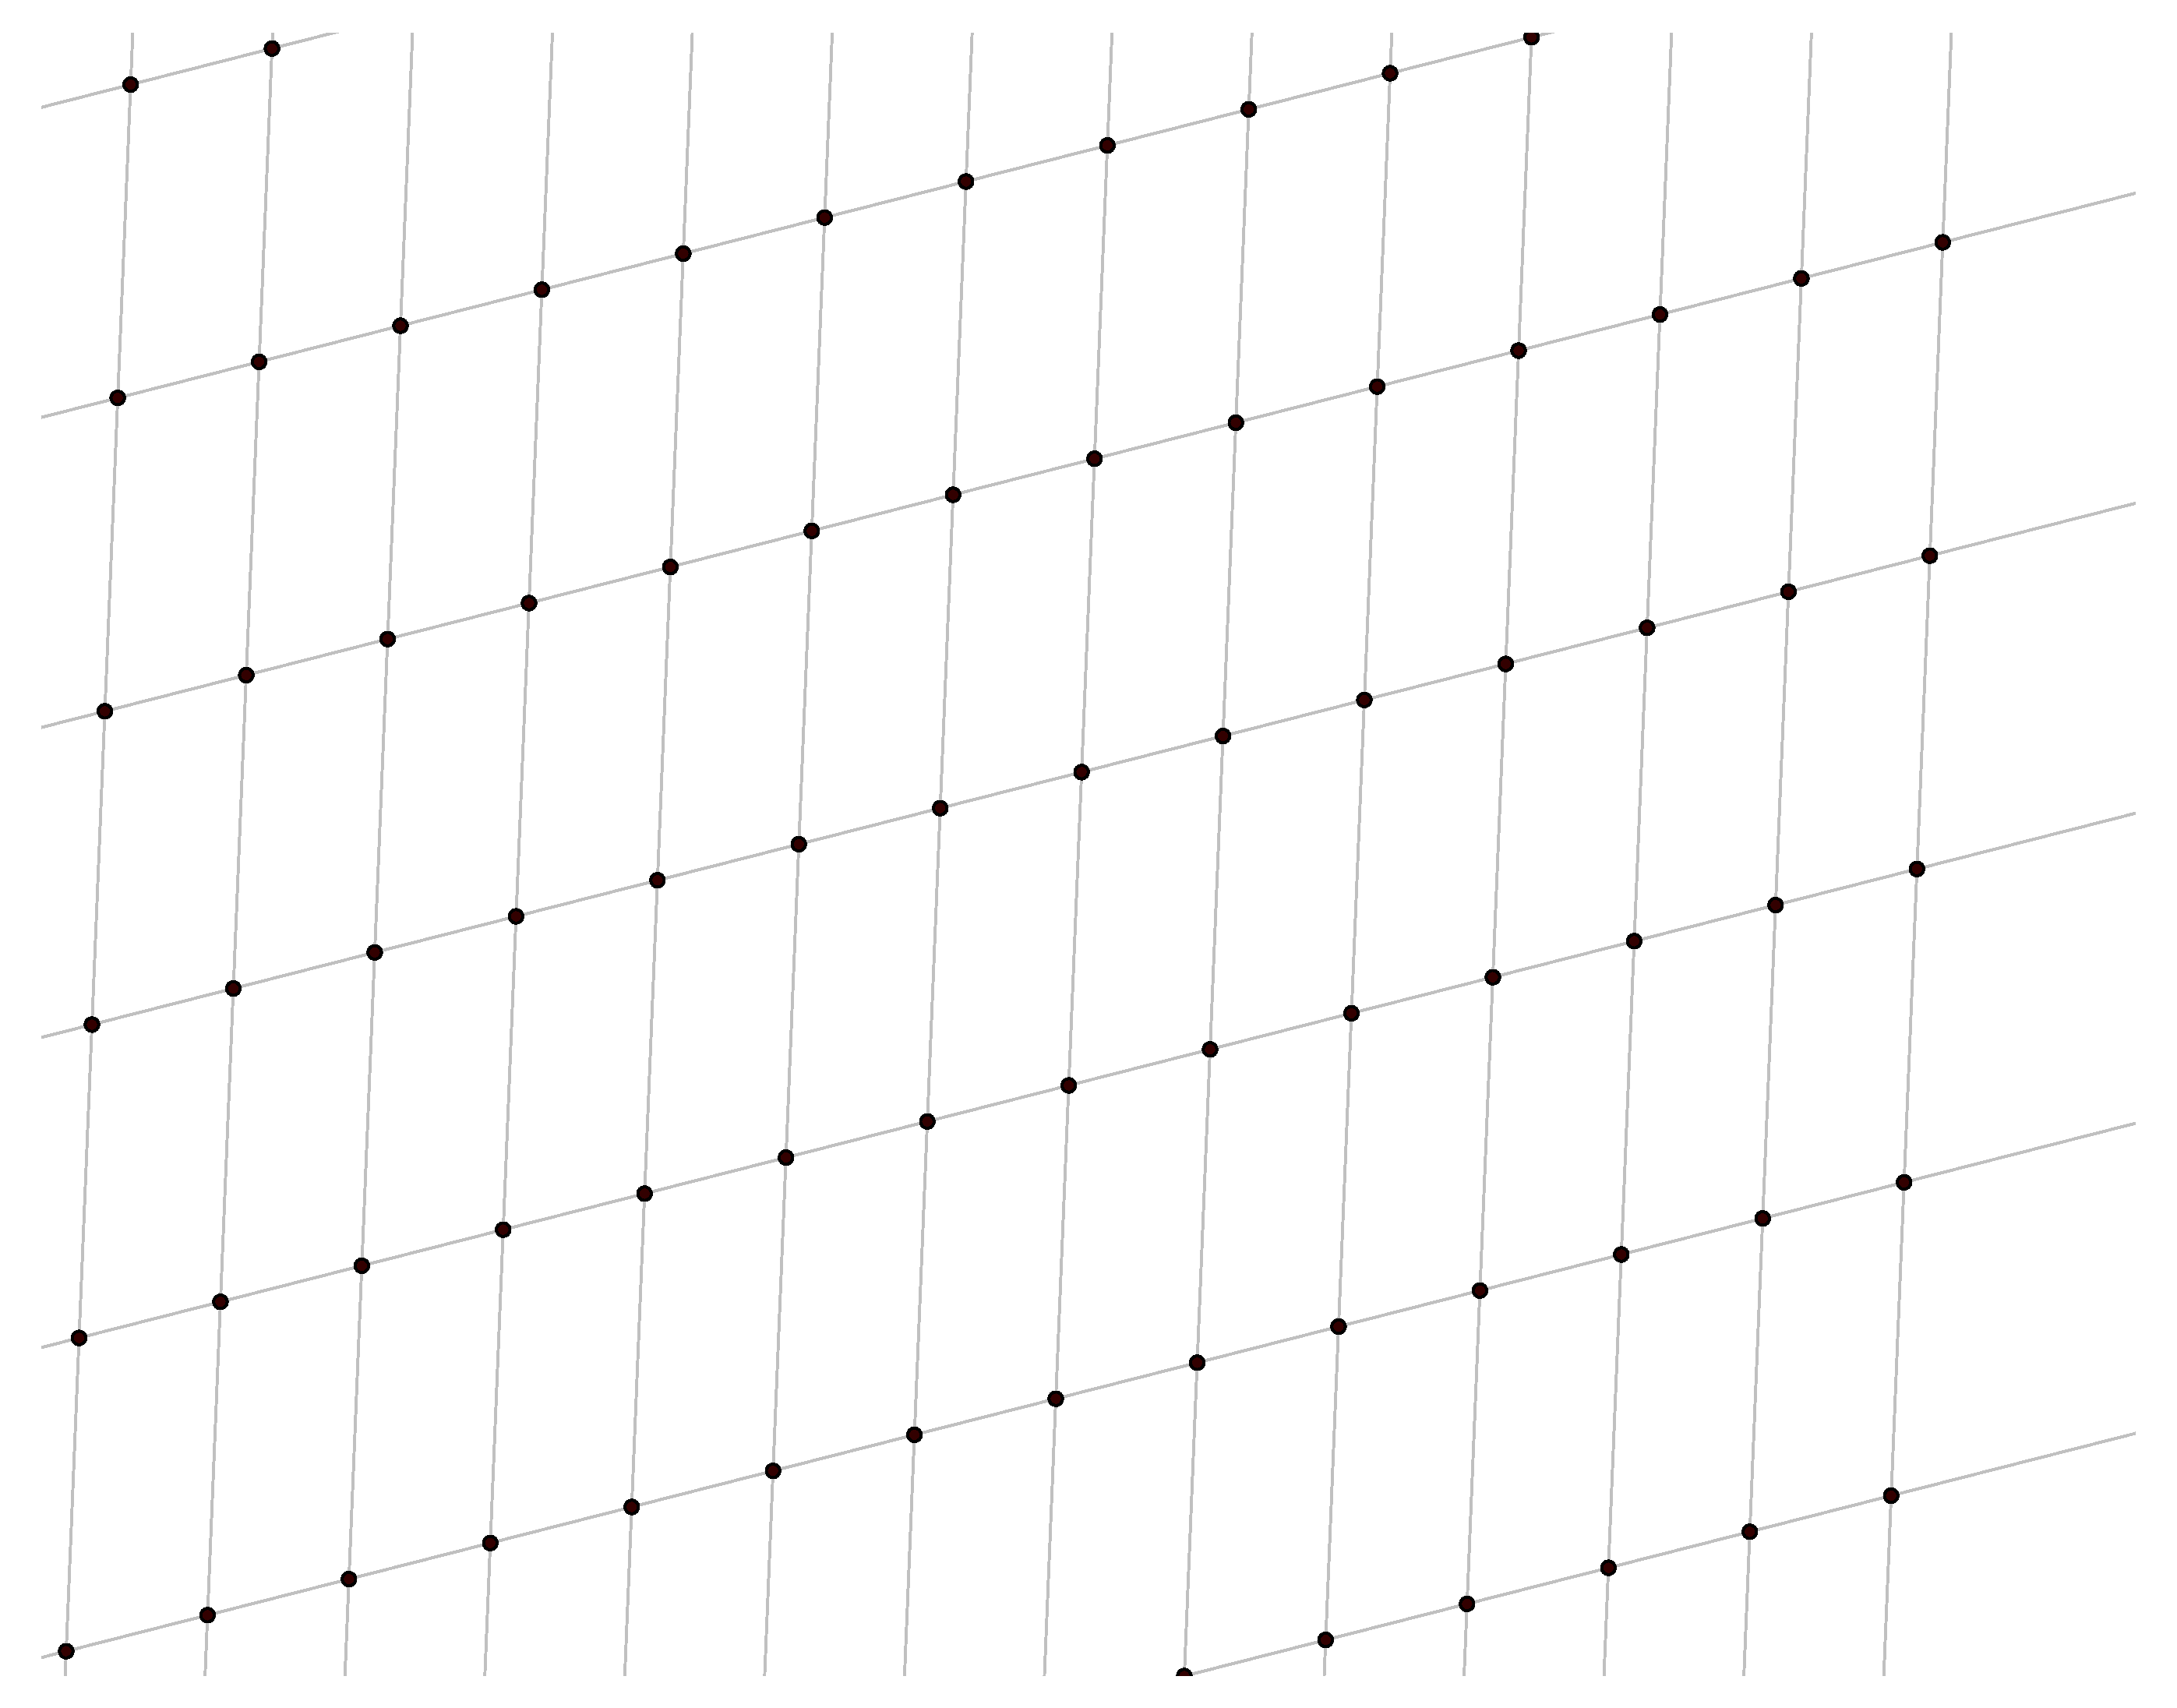
\includegraphics[trim=30 20 180 20, clip, width=\linewidth]{fig/pargrid1.pdf}}
}\end{subfigure}%
\hfill%
\begin{subfigure}{.3\textwidth}
{
	\setlength{\fboxsep}{0pt}%
	\setlength{\fboxrule}{0.5pt}%
	\fbox{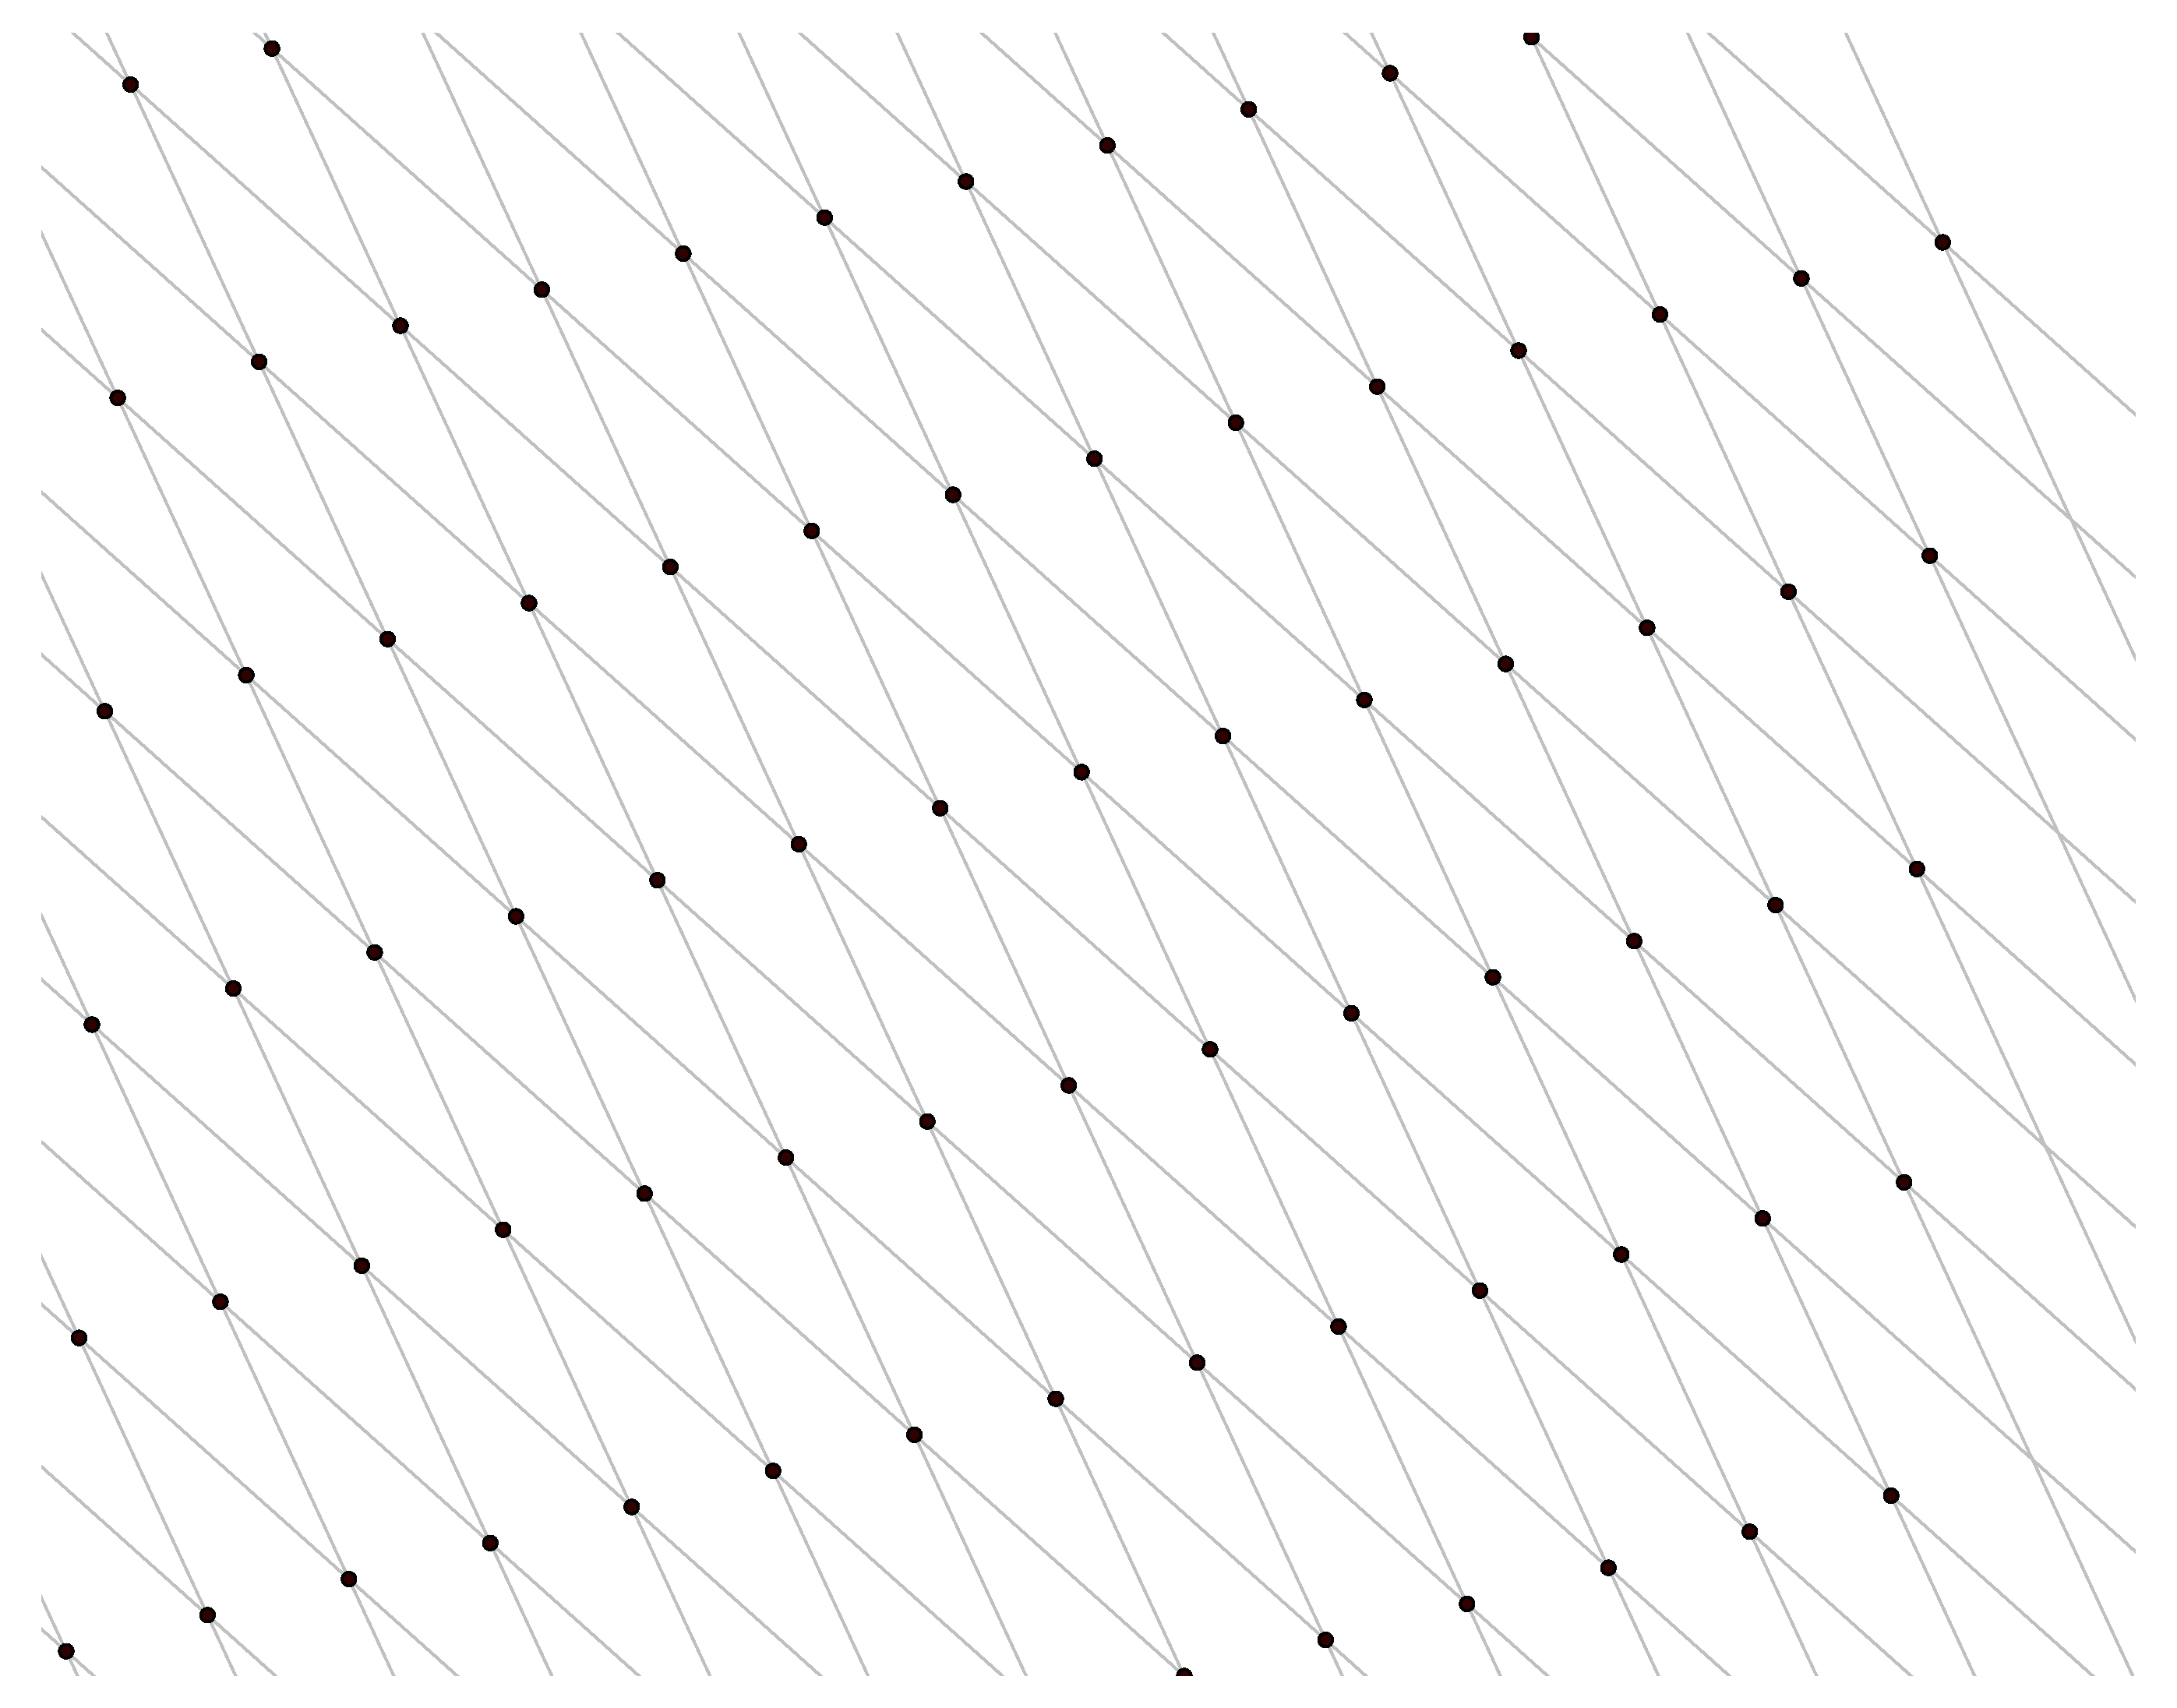
\includegraphics[trim=30 20 180 20, clip, width=\linewidth]{fig/pargrid2.pdf}}
}\end{subfigure}%
\hspace*{\fill}
\caption{Different parallelogram grids for same point dispersion}
\label{fig:par_grid_tilings}
\end{figure}

\FloatBarrier

\section{Measures on grid}
The point density $\rho$ of the points in the parallelogram grid dispersion on the object surface, can be calculated as
\begin{equation}
\rho = \frac{| n_z |}{p^2_l}
\end{equation}

The shortest possible parallelogram side length $l_{\text{min}}$, for any parallelogram grid put on the points, is equal to the nearest neighbor distance of the points.

It can be estimated with the following formula, in function of $p_l$ and the normal vector $\vec{n}$ of a point $p \in P$. It is an estimate of the distance from $p$ to its closest neighbor. The expression gives correct values only when $P$ is locally planar around $p$, and this plane is not too oblique.
\begin{equation} \label{eq:pargrid_lmin}
l_{\text{min}} \approx p_l \, \sqrt{1 + \frac{\min \left\{
	n^2_x, \,
	n^2_y, \,
	1 + 2 \, n_x \, n_y, \,
	1 - 2 \, n_x \, n_y
\right\} }{n^2_z}}
\end{equation}

A threshold condition for how oblique the surface may be is given by this formula
\begin{equation} \label{eq:pargrid_lmin_cond}
|n_z| > \cos \alpha \bigvee
\left[
\left|\frac{n_x}{n_y}\right| < \tan \beta
\bigwedge \left|\frac{n_y}{n_x}\right| < \tan \beta
\bigwedge \tan \left(\tfrac{\pi}{4} - \beta\right) < \left|\frac{n_x}{n_y}\right| < \tan \left(\tfrac{\pi}{4} + \beta \right)
\right]
\end{equation}
where the angles $\alpha$ and $\beta$ are adjusted to some constant. The lower these angles, the more restrictive the condition gets. $\alpha = 50\si{\degree}$ and $\beta = 10\si{\degree}$ were used for the experiments.

To check whether $P$ is locally planar around $p$, a curvature measure as described in \ref{sec:curvature} can be used. This is important since formula \ref{eq:pargrid_lmin} depends only on the normal vector, but on curved surfaces, the normal vectors gradually change direction. So on curved surfaces they reach any intermediate value, even when the nearest neighbor distances don't correspond to the predicted value from the formula.

Depending on how $\alpha$ and $\beta$ are parametrized, formula \ref{eq:pargrid_lmin} gives correct values only in a subset of the cases. Additionally, the ``correct'' values are only approximative predictions of the nearest neighbor distance.

The deduction and proofs for these formulea are given in appendix \ref{sec:proof_pargrid_measures}.



\subsection{Analysis}
Figure \ref{fig:lmin_plot} shows the value $l_{\text{min}}$, in function of the normal vector $\vec{n}$ of the plane. For the color scale a logarithmic scale is used. Blue and green correspond to lower values. The $x$ and $y$ axis of the plot correspond to $n_x$ and $n_y$, the third component is set to $n_z = \sqrt{1 - n^2_x - n^2_y}$. The plot is symmetric around the X and Y axis. The origin point $(0, 0)$ corresponds to $\vec{n} = \transpose{(0, 0, 1)}$, that is, the plane is perpendicular to the camera ray and has a square grid dispersion. Then $l_{\text{min}} = 1$, the side length of the square. For the points on either axis, the plane is turned on one direction only, resulting in a rectangular grid, where the shortest side remains $l_{\text{min}} = 1$. Around the border of the plot, the plane is nearly parallel to the camera rays. When $n_x \approx n_y$, the parallelograms take on a rhombus shape, similar to the second grid shown on figure \ref{fig:par_grid_tilings}. The shortest edge becomes the projection of the squares' diagonal with length $\sqrt{2}$, whereas the projection of its sides results in longer edges.

\begin{figure}[h]
\centering
\includegraphics[width=.4\textwidth]{fig/lmin_plot.pdf}
\caption{Plot of $l_{\text{min}}$ for $\vec{n} = \transpose{\left(x, y, \sqrt{1 - x^2 - y^2}\right)}$ and $p_l = 1$}
\label{fig:lmin_plot}
\end{figure}


\subsection{Verification}
The first (left-side) histogram on figure \ref{fig:relief_nn_hist} was generated by recording for each point $p \in P$ on a point cloud, the distance $d$ to its closest neighbor. (That is, the point $p' \in P$ such that $p' \neq p$ and $\| p - p' \|$ is minimal.) The point cloud $P$ used is a ``relief'' model as described before in section \ref{sec:relief}, projected without occlusion using a parallel projection camera with $p_l = 0.01$.

Two clusters form around $0.01$ for parts of the surface that are near-parallel to the camera rays, and around $0.0115$, where the surface is more oblique in both directions. Since the surface is not everywhere locally planar the histogram does not form sharp spikes.

For the second histogram the values $l_{\text{min}}$ are instead recorded using the normal vectors of the points $p \in P$, and with fixed $p_l = 0.01$. This histogram is generated solely by evaluating the formula \ref{eq:pargrid_lmin}, without looking at the coordinates of the points, or doing a closest neighbor search in $P$.

\begin{figure}[H]
\centering
\begin{subfigure}{.5\textwidth}
	\includegraphics[width=\linewidth]{fig/nn.pdf}
	\caption{Closest neighbor distances on $P$}
\end{subfigure}%
\begin{subfigure}{.5\textwidth}
	\includegraphics[width=\linewidth]{fig/nn_lmin.pdf}
	\caption{Values $l_{\text{min}}(\vec{n})$ on $P$}
\end{subfigure}	
\caption{Comparison of measured closest neighbor distances and $l_\text{min}$ values on relief point cloud.}
\label{fig:relief_nn_hist}
\end{figure}

A similar distribution can be observed on both histograms. The spike at $0.01$ occurs because the camera is placed such that the majority of the surface is approximatively perpendicular to the rays. This confirms the correctness of the formula for $l_{\text{min}}$ for the parallelogram dispersion generated by parallel projection. The similarity of these two histograms also allows for estimation of $p_l$, even when it is not a mode.
 

\subsection{Usage on real point cloud scan}
Figure \ref{fig:ddp_nn_hist} shows the same two histograms, using the ``dessus-de-porte'' scan for $P$ instead of an artificial relief point cloud. The points whose normal vectors fail the threshold condition \ref{eq:pargrid_lmin_cond} or whose curvature is too high are removed prior to taking the histogram.

Some similarity can still be seen, notably the two spikes near $d = 0.0024$ and $d = 0.0034$. Many factors cause the discrepancy between the two histograms:
\begin{itemize}
\item There is some error in the points' positions, which becomes significant in the order of magnitude of nearest neighbor distances. They do not lie exactly on the object surfaces, and do not form a perfect lattice on the surfaces.
\item The scanner does not form exactly the parallelogram lattices as predicted.
\item The scanner rays are not exactly parallel throughout the point cloud.
\item The surface is nowhere completely planar.
\item As explained, the formula \ref{eq:pargrid_lmin} is only correct in a subset of the cases, even when the condition \ref{eq:pargrid_lmin_cond} is applied.
\item The normal vectors are not completely accurate.
\end{itemize}

\begin{figure}[H]
\centering
\begin{subfigure}{.5\textwidth}
	\includegraphics[width=\linewidth]{fig/ddp_nn.pdf}
	\caption{Closest neighbor distances on $P$}
\end{subfigure}%
\begin{subfigure}{.5\textwidth}
	\includegraphics[width=\linewidth]{fig/ddp_nn_lmin.pdf}
	\caption{Values $l_{\text{min}}(\vec{n})$ on $P$}
\end{subfigure}	
\caption{Comparison of measured closest neighbor distances and $l_\text{min}$ values on ``dessus-de-porte'' scan.}
\label{fig:ddp_nn_hist}
\end{figure}



\section{Estimation of projection parameters} \label{sec:estimate_proj_par}
If the point cloud $P$ was generated using a parallel projection camera where the graduation in the $x$ and $y$ directions on the image planes is the same, a constant value $p_l$ exists for the point cloud. This remains true by approximation for small extracts of large 3D scans. In the following the assumption is made that a constant value $p_l$ exists for the entire point cloud.

As shown before, using the properties of the parallelogram grid dispersion and formula \ref{eq:pargrid_lmin}, $p_l$ can be estimated by analyzing the points of the point clouds and their normal vectors. The formula is such that $l_{\text{min}}$ is proportional to $p_l$, and the proportionality constant $m(\vec{n}) = \min \left\{ \cdots \right\}$ is a function of $\vec{n}$. In this formula the coordinate system is such that the camera is at origin, so that a normal vector $\vec{n} = \transpose{(0, 0, 1)}$ points towards it. When $P$ is set in a different coordinate system but the camera pose in it is known, the necessary transformation must be applied. As stated in section \ref{sec:range_image} for range images point clouds the camera is at the right pose.

Assuming that the parallelogram grid covers the entire surface and that the surface is locally planar, $l_{\text{min}}(p)$ can be computed at each point by measuring the distance to the closest neighbor in the point cloud.

A way to estimate $p_l$ is to record $\frac{l_{\text{min}}(p)}{m(\vec{n})}$ for each point and take the median value. The histogram is such that there is one large spike at the correct value $p_l$, and some outliers far off. For point clouds with a high number of points, this estimation remains stable when samples are recorded only for a random subset of the points.
